\section{Introduction}

\begin{figure}
    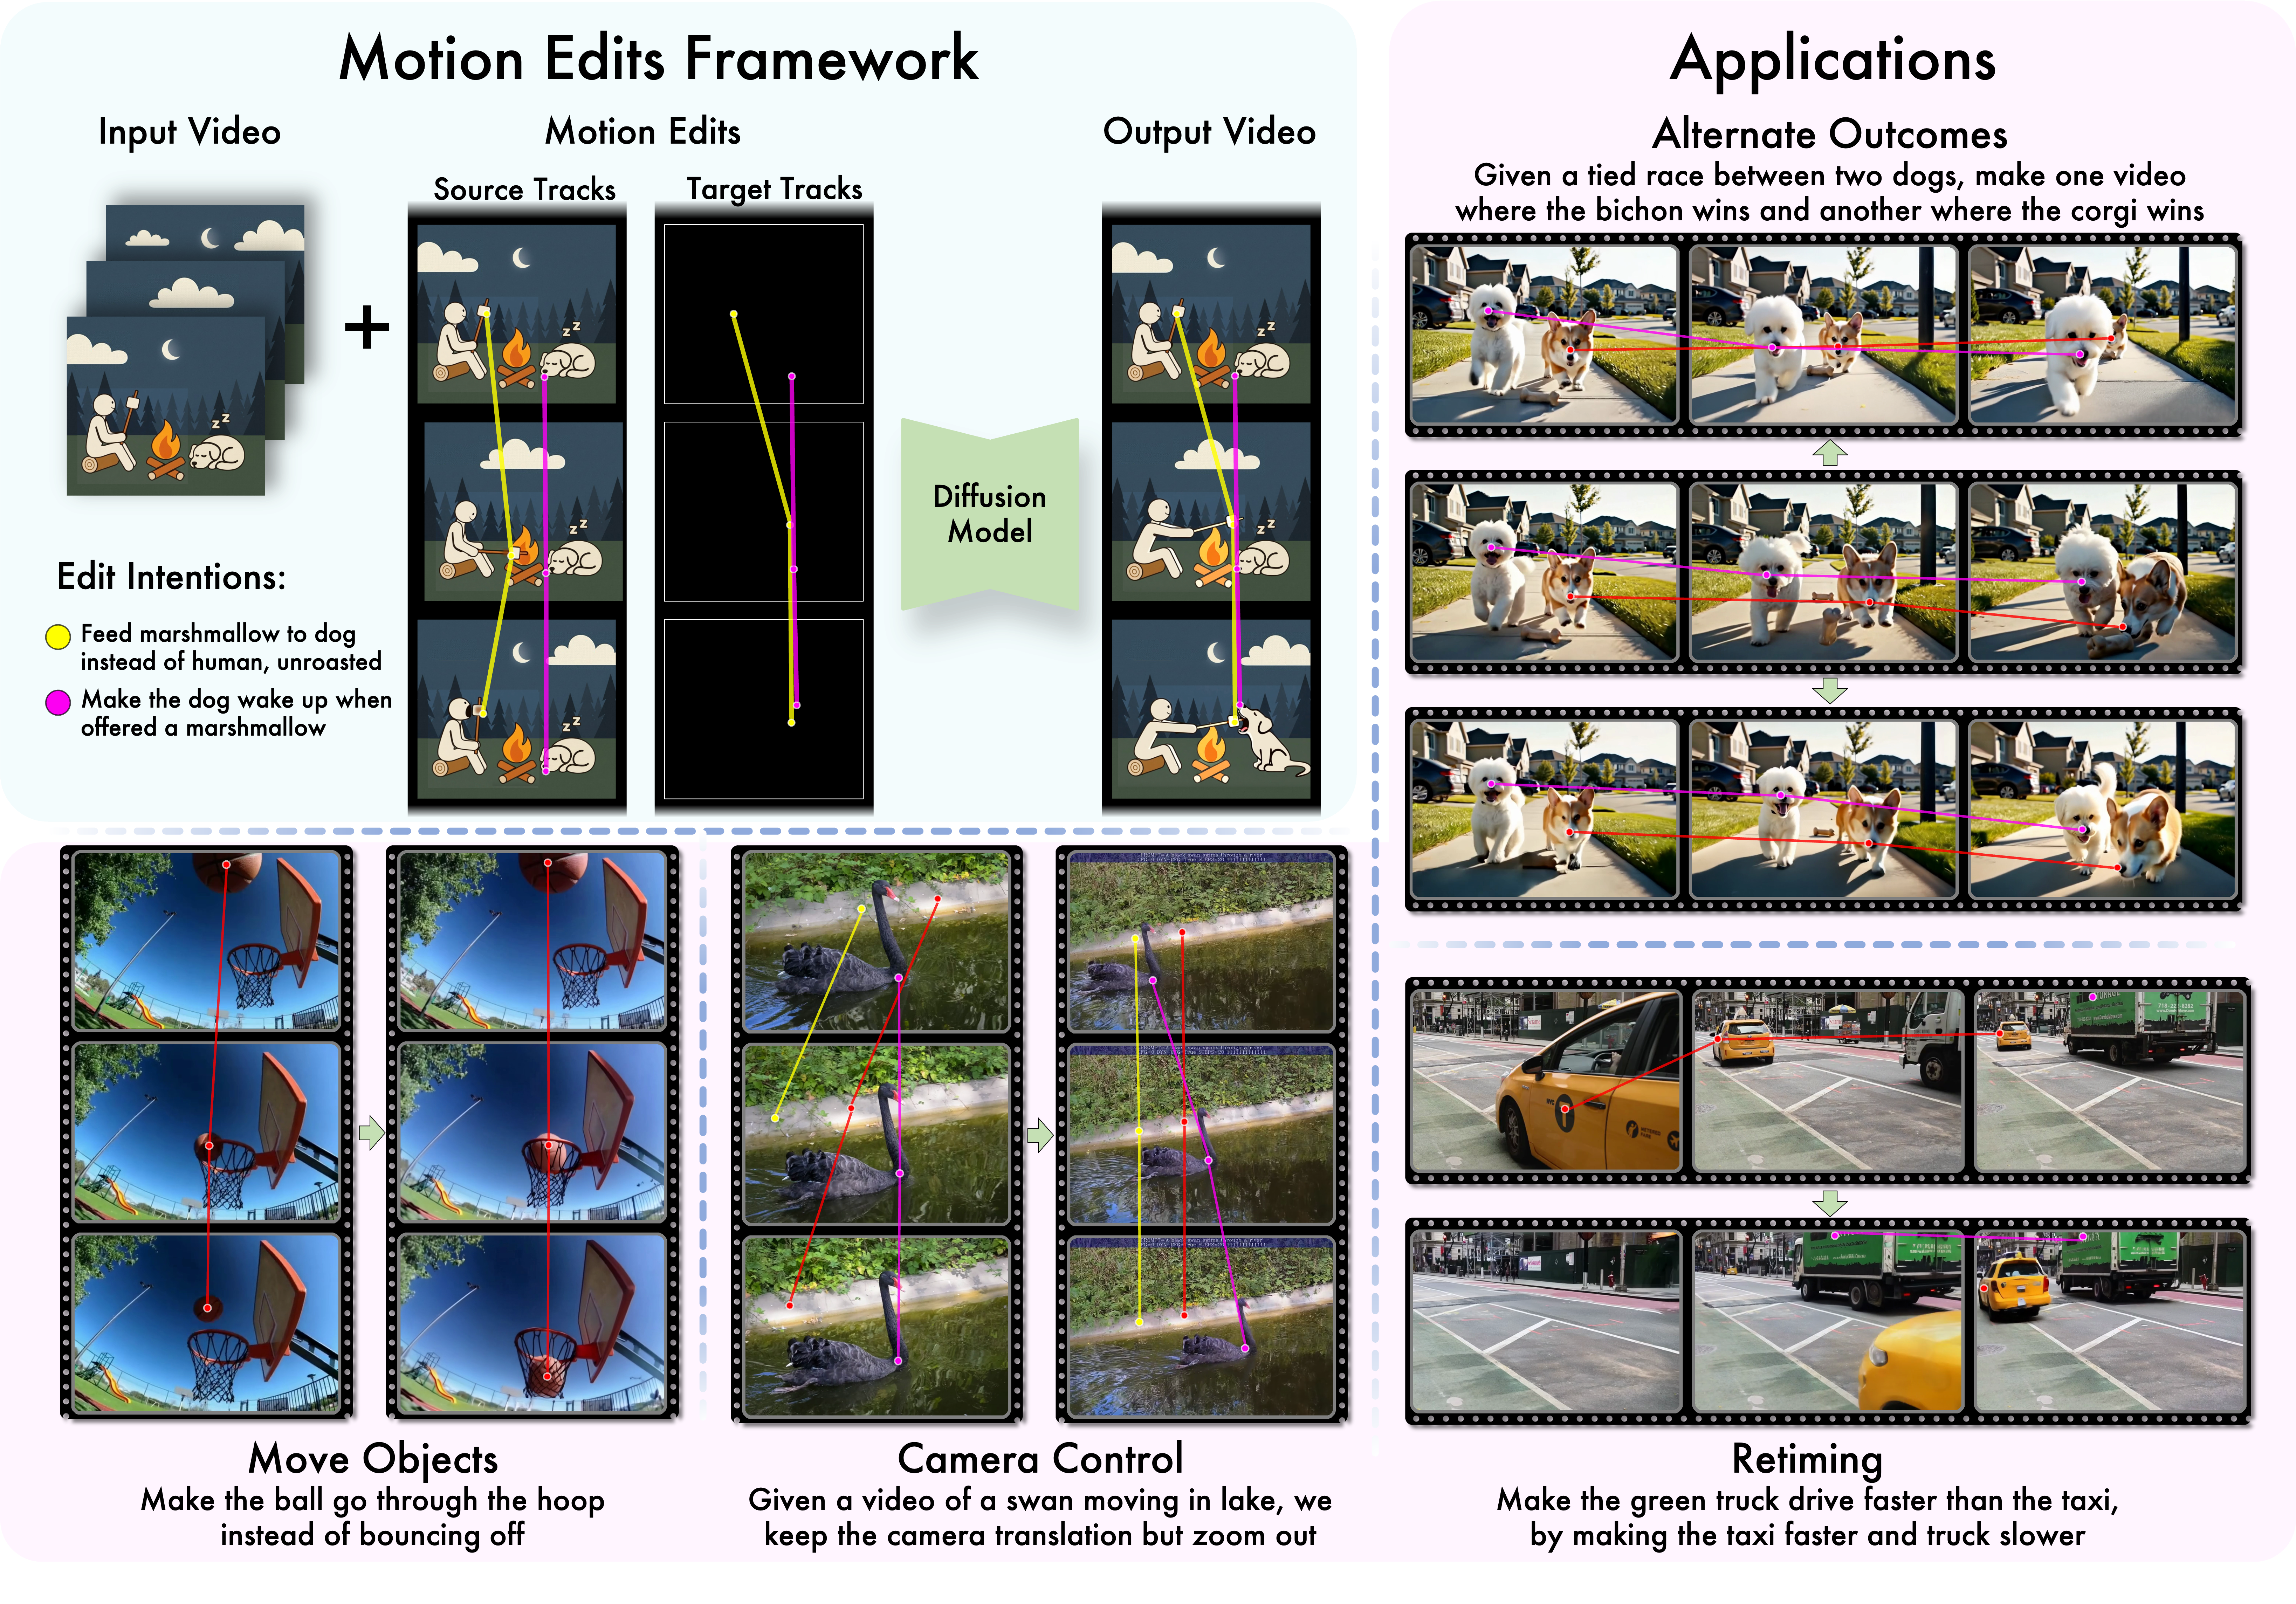
\includegraphics[width=1.0\textwidth]{src/5_MotionV2V/teaserv2.png}
    \captionof{figure}[MotionV2V motion edits framework]{\textbf{Motion Edits Framework:} Users provide an input video along with source motion tracks (colored dots connected by lines, extracted from the input) and target motion tracks (user-specified desired motion). Lines indicate point trajectories while dot presence/absence indicates visibility. Our diffusion model generates an output video matching the target motion. \textbf{Applications:} Our method can edit videos in a true sense, where content is preserved but motion is changed.}
\label{mv2v_fig:teaser}
\end{figure}

Consider filming a climactic race between two dogs: your Corgi and a friend's Bichon. The original video sees the Bichon take the win. After countless recent advances in generative models, does the technology exist to modify this video such that your Corgi is victorious? We propose a method for generalized motion editing in existing user-provided videos that successfully tackles this unsolved problem.

Historically, tackling this problem in the VFX industry has been notably hard. A reshoot for scenes that need substantial changes is usually the necessary option. VFX pipelines can use tricks like retiming and plate stitching, isolated retimes with rotoscoping, or even full-dog CGI replacements. These typically require a high level of skill and large amounts of human hours.

Modern generative models, with their impressive priors, show promise in tackling traditional VFX tasks. In this subfield, current methods for motion editing fall into different categories, each exhibiting significant constraints. Image-to-video (I2V) based approaches like Re-Video~\cite{revideo2024} and Go-with-the-Flow~\cite{gowiththeflow2025} can only generate new video with specified motion conditioned on a single image. Using these on the first frame of a video can give the illusion of video motion control, but have significant drawbacks. For example, content generated in regions that do not appear in that initial frame will be entirely hallucinated, whereas for true video motion editing these regions are known and should remain identical. Re-Video attempts to address this problem by inpainting information from the original video into the edited video, a technique which fundamentally breaks down when the video includes camera movement. Human-specific methods like MotionFollower and MotionEditor can edit motion but are limited to full-body human movements and cannot handle general objects or scenes. Likewise there are also works that allow editing camera trajectories in videos such as ReCapture~\cite{recapture2024} and ReCamMaster~\cite{recammaster2025}. These are not able to edit subject motion.

In this work we introduce motion edits, a new approach for editing videos by controlling the change in motion from the original to the edited video using video diffusion models. While there has been a large amount of successful recent work on appearance-based video editing (i.e.\ transforming visual style while preserving motion structure), motion editing presents a fundamentally different challenge. When editing how objects move within a scene (e.g.\ making a person walk in a different direction), the structural correspondence between input and output videos is broken. This makes the problem harder than appearance-based video editing and renders standard video editing techniques like DDIM inversion ineffective.

Our method addresses this problem, and the limitations of prior work, by acting on the complete video and its motion representation. Users provide an input video along with some sparse tracking points on objects they wish to control; these objects are then automatically tracked throughout the video. Users can then choose to either anchor these points (to preserve original motion) or modify them (to edit the trajectory). For example, in a video of a person walking into a crowd, the system tracks both entities; the user can specify a new direction for the person by altering their tracks while strictly preserving the crowd's original motion. In a more complex edit, the user can change the camera by editing all the points.

Our approach enables diverse video editing capabilities (Figure~\ref{mv2v_fig:teaser}): object motion editing, camera motion editing, control over the timing of content, and successive edits. The motion edits are naturally introduced into the output video and the video model handles plausibility correctly --- e.g.\ when dragging a person's tracking point through an image the model will make the person traverse the image by walking. Our approach requires no manual masking and can handle any type of object, while also maintaining scene consistency even when both object motion and camera movement are edited simultaneously. And in contrast to prior methods, our approach also allows the ability to change when an object appears in the frame. Finally, our model generalizes to vastly different scenes and objects and achieves state-of-the-art performance in quantitative comparisons and human evaluations.

In summary, we propose the following contributions:
\begin{itemize}
\item We identify motion as a powerful control signal for video editing and propose directly editing sparse trajectories extracted from the input video to change the motion of the output video. We define the change between the input and target trajectories as a ``motion edit'' and show that motion edits, coupled with a powerful generative video model, can address several challenging video editing tasks.
\item We present a methodology to train a video diffusion model to generate high quality ``motion counterfactual'' video pairs which have the scene appearance but different motion. As part of this, we also identify sources of data that work well in this training.
\item We propose a new model architecture with careful conditioning on both user-specified video and motion trajectories that generates a motion-edited output.
\end{itemize}

\label{mv2v_sec:intro}
\label{mv2v_sec:method}
